\documentclass{article}
%
% Demo of the mcode package from 
% http://www.mathworks.co.uk/matlabcentral/fileexchange/8015-m-code-latex-package
% Updated 06 Mar 2014
%

\usepackage{graphicx}
\usepackage{wrapfig}
\usepackage{mathtools}
\usepackage{mathrsfs}
\usepackage{enumitem}
\usepackage{pdflscape}
\graphicspath{ {images/} }

% load package with ``framed'' and ``numbered'' option.
\usepackage[framed,numbered,autolinebreaks,useliterate]{mcode}

% something NOT relevant to the usage of the package.
\usepackage{url}
\setlength{\parindent}{0pt}
\setlength{\parskip}{18pt}


% //////////////////////////////////////////////////

\begin{document}

\title{Homework 4 - Optimal Control Systems}
\author{Erivelton Gualter dos Santos, 2703806}
\date{}

\maketitle 

\section{Linear Quadratic Regulator problem}

Plant to be controlled: 
\begin{eqnarray}\label{i1}
\begin{split}
	\dot{x}_1(t) &= x_2(t) \\
	\dot{x}_2(t) &= -x_2(t) + x_2(t) + u(t)
\end{split}
\end{eqnarray}

Performance measure:
\begin{equation}
J = 10{x_ 1}^2(T) + \frac{1}{2}\int_{0}^{T} \left[ {x_ 1}^2(t) + 2{x_ 2}^2(t) + u^2(t)\right] dt
\end{equation}

As the general regulation objective is:
\begin{equation}
J = \frac{1}{2}{x(t_f)}^THx(t_f) + \int_{t_0}^{t_f} \frac{1}{2}\left[ {x^T(t_f)}Q(t)x(t_f) + {u^T(t)}R(t)u(t) \right] dt
\end{equation}

Therefore the LQR parameters for the given performance measure is:
\begin{equation*}
H = 
\begin{bmatrix}
20  & 0 \\
0 & 0
\end{bmatrix}
\:\:\: 
Q = 
\begin{bmatrix}
1 & 0 \\
0 & 2
\end{bmatrix}
\:\:\: 
R = 1
\end{equation*}

\begin{center} \begin{figure} 
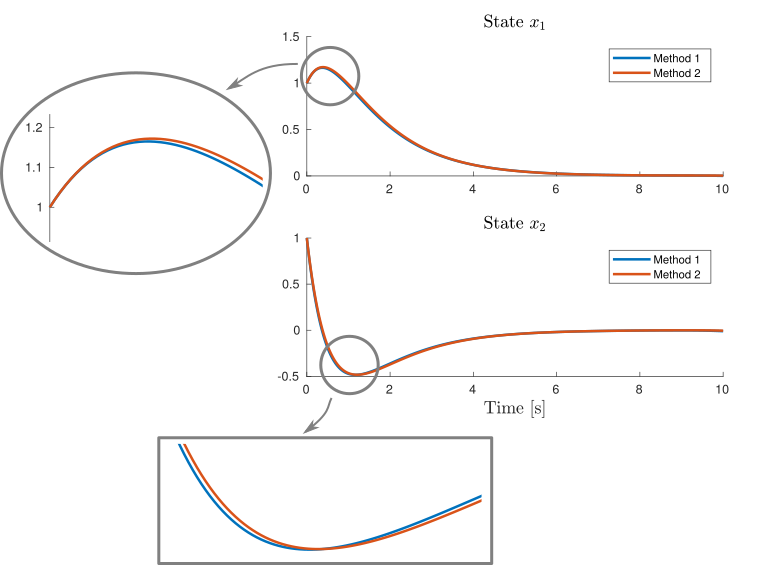
\includegraphics [width=4.5in]{states.png}
\caption{Optimal Control Law plots for two different solving methods}
\end{figure}  \end{center}

\begin{center} \begin{figure} 
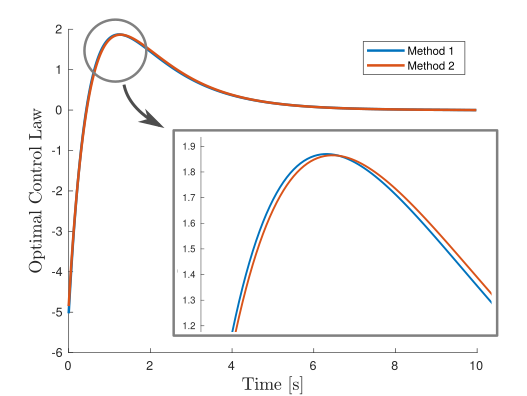
\includegraphics [width=4.5in]{controllaw.png}
\caption{States plots for two different solving methods}
\end{figure}  \end{center}

\begin{center} \begin{figure}[h]
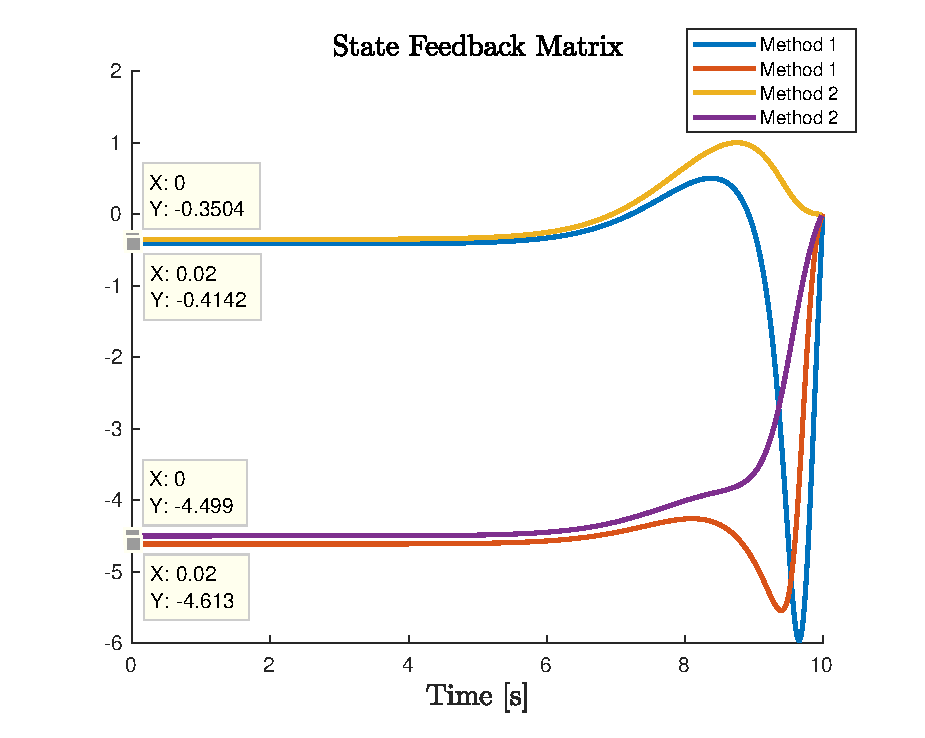
\includegraphics [width=4.5in]{SFM.eps}
\caption{State Feedback Matrix}
\end{figure}  \end{center}

As showed in figures 1 and 2, the states and the optimal control law is very similar with a insignificant difference between each other. Also, it happens for the steady state values of State Feedback matrix. However, the shape of the function to reach the steady state is different from each other as represented in figure 3.

\pagebreak

\begin{lstlisting}
% Book: Optimal Control Theory: An introduxtion by Donald E. Kirk
%
% Erivelton Gualter, 02/08/2018
% LQR

clear all, close all, clc

% Plant
A = [0 1; -1 2];
B = [0; 1];

% LQR Parameters
H = [20 0; 0 0];
Q = [1 0; 0 2];
R = 1;

% Simulation Parameters
T = 10;
dt = 0.02;
t = 0:dt:T; 
X0 = [1; 1];

%% Riccati Approach
N = length(t);
K(:,:,N) = H;
for k=N:-1:2
    Kd(:,:,k) = -Q + K(:,:,k)*B*inv(R)*B'*K(:,:,k) - K(:,:,k)*A - A'*K(:,:,k);
    K(:,:,k-1) = K(:,:,k) - Kd(:,:,k)*dt;
end
ktemp = K(1,1,:); K11(:) = ktemp(:,:,:);
ktemp = K(1,2,:); K12(:) = ktemp(:,:,:);
ktemp = K(2,1,:); K21(:) = ktemp(:,:,:);
ktemp = K(2,2,:); K22(:) = ktemp(:,:,:);

X = X0;
for k=1:N-1

    u(k)  = -inv(R)*B'*K(:,:,k)*X(:,k);
    SFM(:,k) = -inv(R)*B'*K(:,:,N-k+1);
        
    XD = A*X(:,k) + B*u(k);
    
    X(:,k+1) = X(:,k) + XD*dt;    
end

%%
[Ad, Bd] = c2d(A,B, dt);
% Ad = A; Bd = B;
N = T/dt+2;
P(:,:,1)= eye(2);    
for k=2:N-1
    S = R + Bd'*P(:,:,k-1)*Bd;
    F(:,:,N-k) =  -( inv(S) * Bd' * P(:,:,k-1) * Ad );
    P(:,:,k) = (Ad + Bd*F(:,:,N-k))'*P(:,:,k-1)*(Ad + Bd*F(:,:,N-k)) + F(:,:,N-k)'*R*F(:,:,N-k) + Q;
end

Xric = X0;
for k=1:N-2

    uric(k) = F(:,:,k)*Xric(:,k);
    
    XD = A*Xric(:,k) + B*uric(k);
    
    Xric(:,k+1) = Xric(:,k) + XD*dt;
end

%%
f1 = figure;
ax1 = subplot(211); hold on; plot(t, X(1,:), t, Xric(1,:),'LineWidth',2);
ax2 = subplot(212); hold on; plot(t, X(2,:), t, Xric(2,:),'LineWidth',2);
title(ax1, 'State $x_1$','Interpreter','latex','FontSize',14); 
title(ax2, 'State $x_2$','Interpreter','latex','FontSize',14);   
legend(ax1, 'Method 1', 'Method 2');
legend(ax2, 'Method 1', 'Method 2');
xlabel('Time [s]', 'Interpreter','Latex', 'FontSize',14);
saveFigureToPdf('fig1',f1);
    
f2 = figure; hold on;
tu = t(1:end-1);
plot(tu, u, tu, uric,'LineWidth',2);
title('State $x_1$','Interpreter','latex','FontSize',14); 
legend('Method 1', 'Method 2');
xlabel('Time [s]', 'Interpreter','Latex', 'FontSize',14);
ylabel('Optimal Control Law', 'Interpreter','Latex', 'FontSize',14);
saveFigureToPdf('fig2',f2);
\end{lstlisting}

You can access the code at: https://github.com/EriveltonGualter/EEC-744-Optimal-Control-Systems

\pagebreak


\section{Linear Quadratic Tracking problem}

The performance measure for the LQ tracking can be written as:
\begin{equation*}
J = \frac{1}{2}{(Cx(t_f)-r(t_f))}^TH(Cx(t_f)-r(t_f)) + \int_{t_0}^{t_f} \frac{1}{2}\left[ {(Cx(t_f)-r(t_f))}^TQ(t)(Cx(t_f)-r(t_f)) + {u^T(t)}R(t)u(t) \right] dt
\end{equation*}

As we desire to track the following state, we need to choose the LQ tracker parameters to perform this task.

$$ r = [sin(t) \frac{t}{2}]^T $$

For C=H=Q=Identity we have the following state feedback matrix:

\begin{center} \begin{figure}[h]
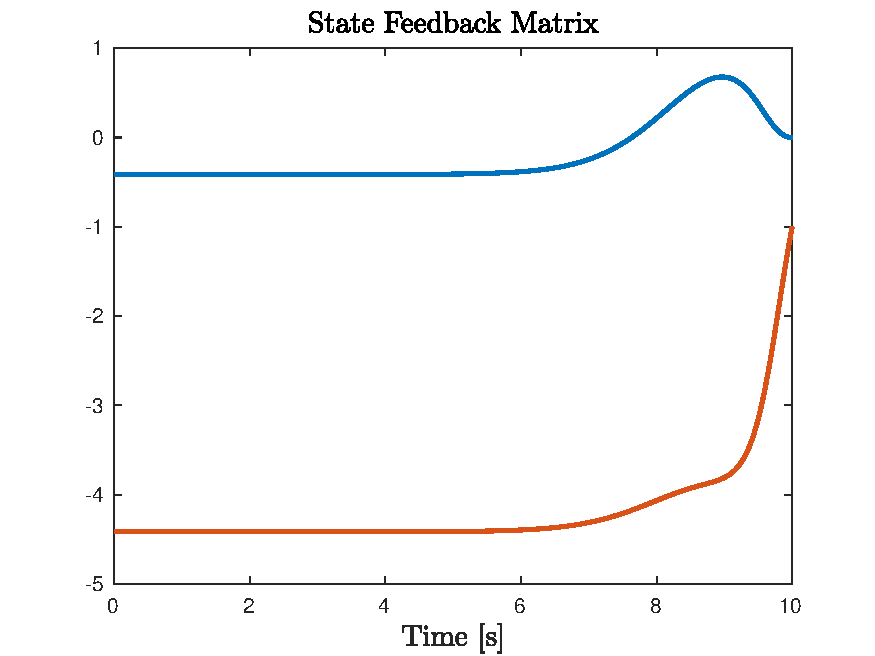
\includegraphics [width=4.5in]{lq}
\caption{State Feedback Matrix}
\end{figure}  \end{center}
Note that if C=I and r=0, it will perform as a Linear Quadratic Regulator problem
\begin{center} \begin{figure}[h]
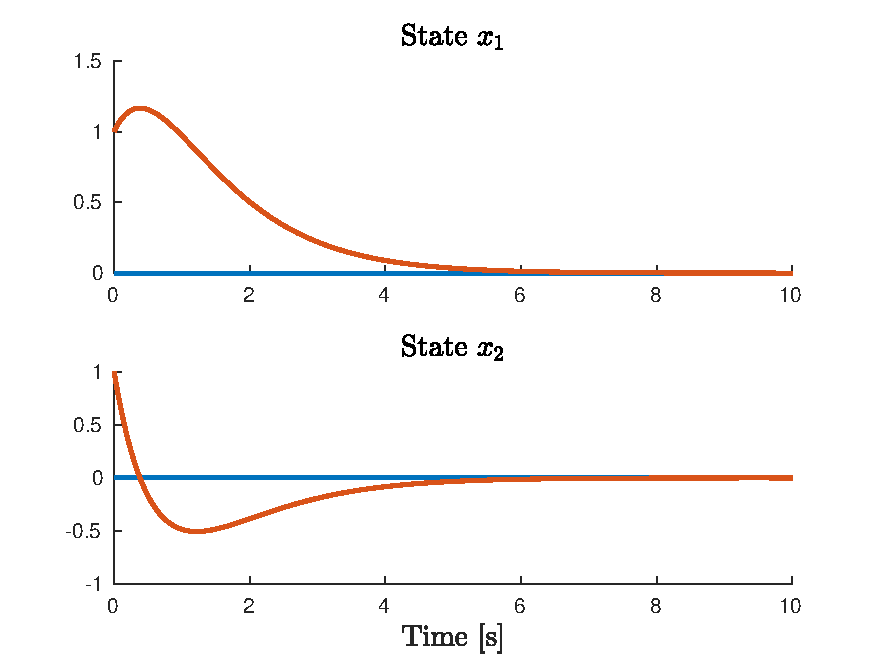
\includegraphics [width=4.5in]{lq2}
\caption{State Feedback Matrix}
\end{figure}  \end{center}
For the following parameters:
\begin{equation*}
H = 
\begin{bmatrix}
1  & 0 \\
0 & 1
\end{bmatrix}
\:\:\: 
Q = 
\begin{bmatrix}
10 & 0 \\
0 & 0
\end{bmatrix}
\:\:\: 
R = 1
\end{equation*}
The following plots contains the State Feedback Matrix, States and Optimal Control Input. Due to the characteristic of the plant and the desired trajectory, it is not possible to find parameters to track both states. You can see that the states has a shift for the states $x_1$. For any other value of C, H, Q will not be enough to track both states.

\begin{center} \begin{figure}[h]
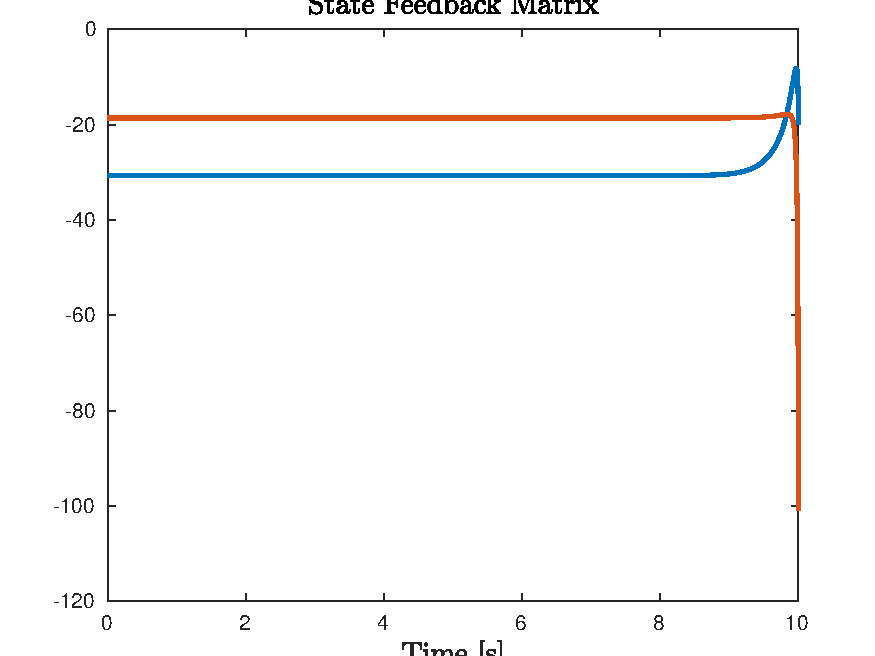
\includegraphics [width=4.5in]{sfm2}
\caption{State Feedback Matrix}
\end{figure}  \end{center}

\begin{center} \begin{figure}[h]
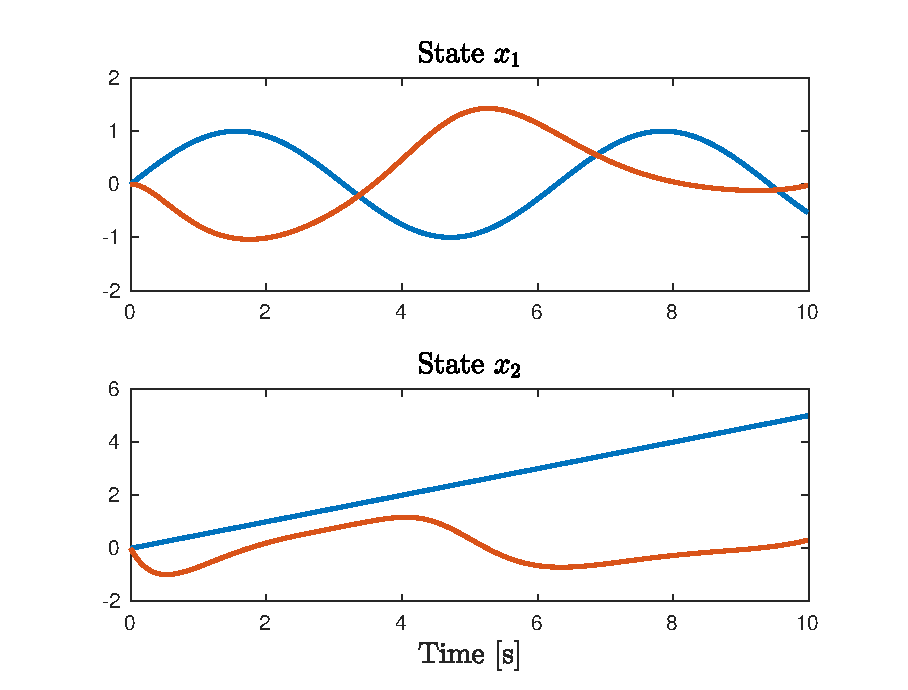
\includegraphics [width=4.5in]{states.eps}
\caption{State Feedback Matrix}

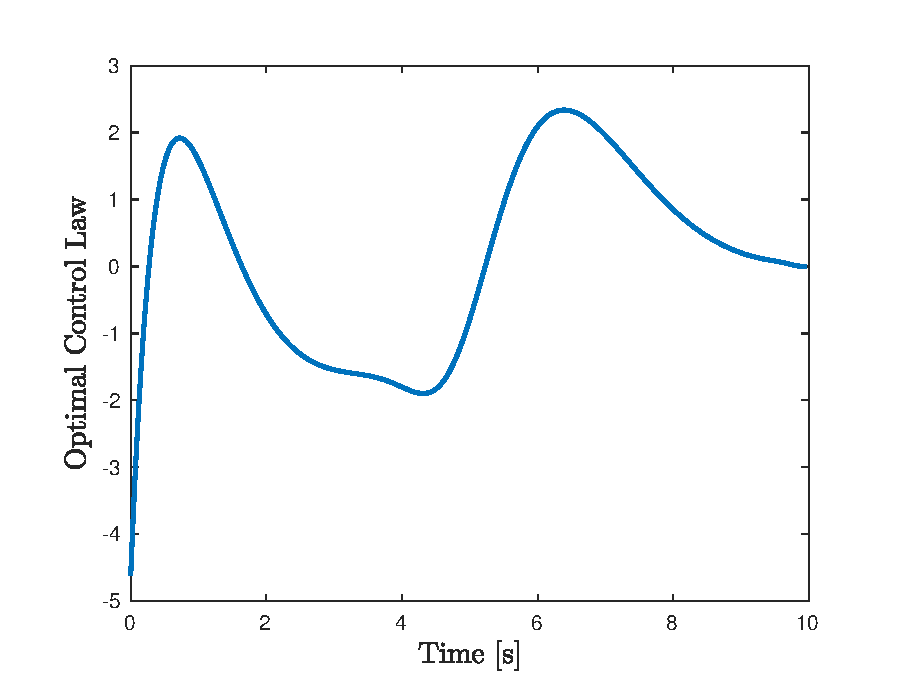
\includegraphics [width=4.5in]{control.eps}
\caption{State Feedback Matrix}
\end{figure}  \end{center}

\pagebreak

\pagebreak

\begin{lstlisting}
clear all, close all, clc

% Plant
A = [0 1; -1 2];
B = [0; 1];

% Simulation Parameters
T = 10;
dt = 0.001;
t = 0:dt:T; 
X0 = [1; 1];

% LQR Parameters
H = [1 0; 0 1];
Q = [10 0; 0 2];
R = 1;
C = [10 1; 1 10];
r = [sin(t); t/2];
% r = zeros(2,length(t))

%% Riccati Approach
N = length(t);
K(:,:,N) = C'*H*C;
V(:,:,N) = C'*H*r(end);
for k=N:-1:2
    
    Kd(:,:,k) = -C'*Q*C + K(:,:,k)'*B*inv(R)*B'*K(:,:,k) - K(:,:,k)*A - A'*K(:,:,k);
    Vd(:,:,k) = -(A'-K(:,:,k)'*B*inv(R)*B')*V(:,:,k) - C'*Q*r(:,k);
    
    K(:,:,k-1) = K(:,:,k) - Kd(:,:,k)*dt;
    V(:,:,k-1) = V(:,:,k) - Vd(:,:,k)*dt;
end
ktemp = K(1,1,:); K11(:) = ktemp(:,:,:);
ktemp = K(1,2,:); K12(:) = ktemp(:,:,:);
ktemp = K(2,1,:); K21(:) = ktemp(:,:,:);
ktemp = K(2,2,:); K22(:) = ktemp(:,:,:);

X = X0;
for k=1:N-1

    u(k)  = -inv(R)*B'*K(:,:,k)*X(:,k);
    SFM(:,N-k+1) = -inv(R)*B'*K(:,:,N-k+1);
    
    XD = A*X(:,k) + B*u(k);
    
    X(:,k+1) = X(:,k) + XD*dt;    
end

% Performance Measure (calc cost)
for k=1:N-2
    J(k) = X(:,end)'*H*X(:,end)/2 + (X(:,k)'*Q*X(:,k) + u(k)*R*u(k))/2;
end

% Performance Measure (calc cost)
for k=1:N-2
    J(k) = (C*X(:,end)-r(:,end))'*H*(C*X(:,end)-r(:,end))/2 + ((C*X(:,k)-r(:,end))'*Q*(C*X(:,k)-r(:,k)) + u(k)*R*u(k))/2;
end

%%
fig1 = figure
ax1 = subplot(211); hold on; plot(t, r(1,:),'LineWidth',2); plot(t, X(1,:),'LineWidth',2);
ax2 = subplot(212); hold on; plot(t, r(2,:),'LineWidth',2); plot(t, X(2,:),'LineWidth',2);
title(ax1, 'State $x_1$','Interpreter','latex','FontSize',14); 
title(ax2, 'State $x_2$','Interpreter','latex','FontSize',14);   
xlabel('Time [s]', 'Interpreter','Latex', 'FontSize',14);
saveFigureToPdf('lq_lqr',fig1);


fig = figure
plot(t(2:end), SFM(:,2:end),'LineWidth',2);
xlabel('Time [s]', 'Interpreter','Latex', 'FontSize',14);
title('State Feedback Matrix', 'Interpreter','Latex', 'FontSize',14);
saveFigureToPdf('stm2',fig);

figure; plot(J)
\end{lstlisting}


\end{document}
